\section{Choix technologiques}
\label{section:choixTechnologiques}

\subsection*{Choix de l'environnement de programmation}

Parmi la myriade de langages de programmations (avec leurs différentes plate-formes logicielles existantes) possibles, nous avons opté pour le langage JavaScript et la plate-forme Node.js pour toutes les parties de notre solution (\Gls{backend}, \Gls{frontend} et \Gls{cli}). \\

Ce langage ne vous est peut-être pas tout à fait inconnu en effet, il est souvent utilisé conjointement avec les interfaces HTML du côté client. Le JavaScript est souvent mal considéré par les utilisateurs, lesquels mettent en cause ses difficultés. \\

Néanmoins, ce langage riche n’en reste pas pour la cause dépourvu d’avantages et pour illustrer ce panel, nous n'en citerons que quelques points : JavaScript est un langage basé sur les événements ; il permet ainsi de mettre à jour dynamiquement l’interface qu’il assiste, et c’est notamment le cas pour la quasi-totalité des fameuses messageries instantanées utilisées partout.\\

Node.js nous permet désormais, à l'instar du PHP, d'écrire du code JavaScript du côté serveur qui servira à répondre aux requêtes du client, tout en bénéficiant des avantages du JavaScript. \\

% width=\textwidth,height=\textheight,keepaspectratio
% height=0.24\textheight semble être la seule solution
% car scale fait n'importe quoi
\begin{figure}[H]
    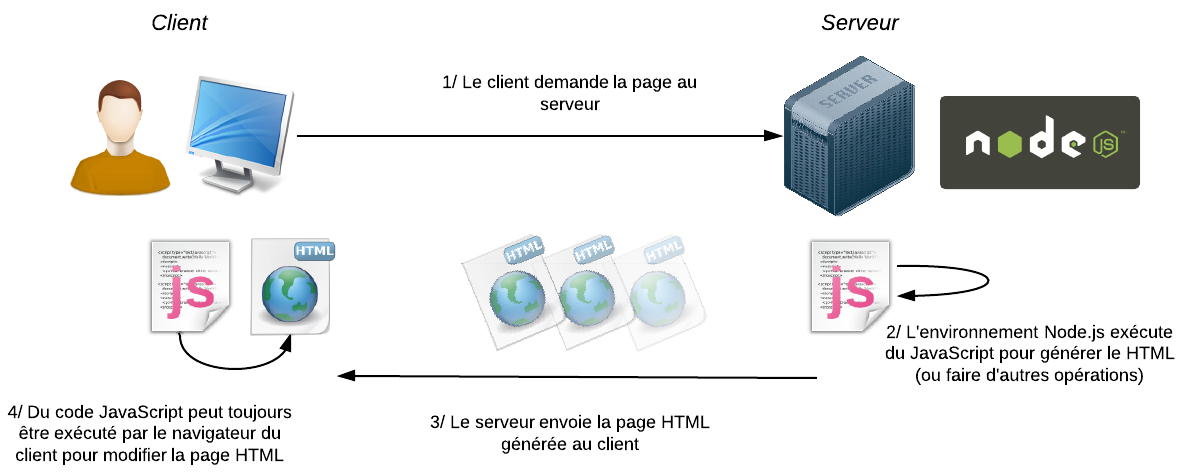
\includegraphics[width=\textwidth,height=0.24\textheight,keepaspectratio]{images/SchemaNodejs.png}
    \centering
    % Un caption alternative pour ne pas afficher la ref dans la table des figures
    \caption[Du JavaScript aussi bien côté serveur que client]{Du JavaScript aussi bien côté serveur que client~\cite{NodejsIllustrations}}
    \label{pic:WhatIsNodeJs}
\end{figure}

Deux points sont élémentaires pour expliquer l'intérêt et la rapidité de Nodejs : le moteur Javascript V8 et son fonctionnement non bloquant. \\

Ce moteur, développé par Google, très performant et optimisé propose la compilation à la volée (en anglais, JIT , just-in-time compilation) , approche hybride entre la compilation et l'interprétation, dont nous pouvons schématiser leur mode de fonctionnement individuel par la figure suivante :
\begin{figure}[H]
    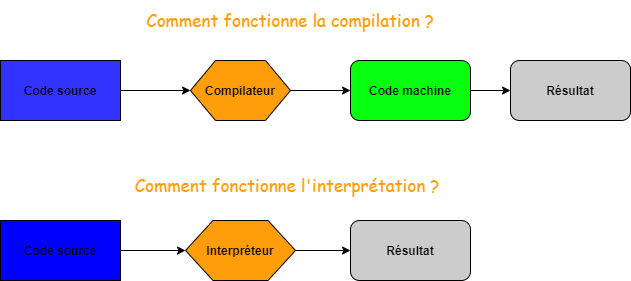
\includegraphics[width=\textwidth,height=0.2\textheight,keepaspectratio]{images/compilationVSinterpretation.png}
    \centering
    \caption{Compilation et interprétation - mode de fonctionnement}
\end{figure}

Malheureusement, la compilation et l'interprétation ont chacune leurs qualités et défauts, que l'on peut synthétiser en 4 grand points :
\begin{itemize}
    \item Une fois compilé, on ne peut plus changer le programme (contrairement à l'interprétation)
    \item En cas d'erreur(s) dans le programme, la compilation les affiche dans la phase "compilation" contrairement à l'interprétation qui les affiche à l'exécution. 
    \item La compilation permet d'optimiser les performances d'un programme (car disposant de l'intégralité du code source au départ) mais nécessite un certain temps pour traduire le programme en code machine.
    \item L'interprétation possède moins d'étapes que la compilation.
\end{itemize}

Dans tout système, il existe des tâches coûteuses en temps : des appels à la base de données, etc.
Dans un mode de fonctionnement bloquant, il convient d'attendre la fin de ces taches avant de réaliser autre chose. Ceci est un gâchis dans la mesure où des tâches moins gourmandes en temps sont ainsi bloquées. Node.js permet, par son mode de fonctionnement non bloquant, des gains de performances, comme illustré ci-dessous.

% width=\textwidth,height=\textheight,keepaspectratio
\begin{figure}[H]
    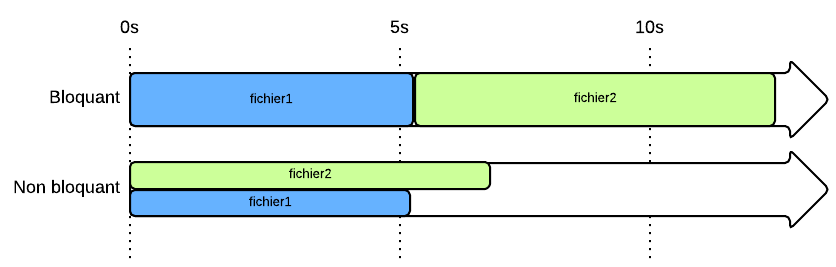
\includegraphics[width=\textwidth,height=0.19\textheight,keepaspectratio]{images/ComparaisonBloquantOuNon.png}
    \centering
    % Un caption alternative pour ne pas afficher la ref dans la table des figures
    \caption[Bloquant/non-bloquant : un exemple pour l'illustrer]{Bloquant/non-bloquant : un exemple pour l'illustrer~\cite{NodejsIllustrations}}
    \label{pic:BloquantOrNot}
\end{figure}

\pagebreak

\subsection*{Choix des frameworks}

% Sans doute une référence à mettre
Un framework peut être considéré comme une boite à outils très pratique nous permettant de développer une application conséquente en disposant de fonctionnalités et d'une structure de base. Nous pouvons citer 2 avantages majeurs à son usage : 
\begin{itemize}
    \item Une architecture spécialement prévue (et souvent éprouvée) pour résoudre des classes de problèmes précises permettant ainsi une maintenabilité / évolutivité  de l'application
    \item Une standardisation de la programmation permettant ainsi d'interchanger, d'injecter et/ou réutiliser du code existant pour ne pas "réinventer la roue".
\end{itemize}
Dès lors, ce choix, qui possède aussi son lot d'inconvénients, ne saurait être pris à la légère car il constitue le squelette de l'application. C'est pourquoi vous pourrez retrouver ci dessous une liste non-exhaustive des frameworks (dans les tables \ref{table:compFrameworksFrontend}, \ref{table:compFrameworksAPI} et \ref{table:compFrameworksCLI}) que nous avons étudié ainsi que les critères retenus pour les départager. \\

\noindent\textbf{Critères - [M]auvais, [S]ufficient, [B]on}

\begin{itemize}
    \item[\textbf{Doc}] Documentation : \\
    La présence d'une documentation suffisamment claire et explicite pour répondre aux principales questions sur son utilisation.
    La qualifier n'est pas une tâche aisée puisque souvent soumise exclusivement à notre subjectivité personnelle : en effet, des mesures quantitatives tel que le ratio entre le nombre de lignes de commentaires (\textbf{CLOC}) et le nombre total de lignes de code (\textbf{LOC}) n'aident pas car quantité n'est pas synonyme de qualité .. 
    \item[\textbf{Fcts}] Fonctionnalités : \\
    Le nombre de fonctions utilitaires ainsi que de leur degré réciproque d'utilité / de praticité perçu par les utilisateurs. Un choix binaire ne peut dès lors pas s'appliquer : une solution minimaliste en nombre de fonctionnalités pourrait davantage répondre à nos besoins.
    \item[\textbf{Maint}] Maintenabilité d'une application créée avec ce framework : \\
    Il s'agit du degré de facilité avec laquelle la maintenance du code est accomplie. Plusieurs paramètres dont la structure et la complexité du code impactent ce critère. Il s'agit dès lors de ne pas négliger ce critère car rien n'exclut l'ajout de nouvelles fonctionnalités ou la découverte de bugs à l'avenir.
    \item[\textbf{Pop}] Popularité : \\
    Le fait d'être connu et d'être utilisé par un grand nombre d'utilisateurs.
    Puisque notre solution est entièrement basée sur Node.js, nous pouvons consulter des données publiques du registre par défaut (NPM) notamment par des sites comme \href{https://www.npmtrends.com/}{NPM Trends}.
    \item[\textbf{Perfs}] Performances : \\
    Elles se mesurent en fonction du temps de réponse à une requête client.
    Il convient cependant d'être prudent avec cette explication simpliste : certaines requêtes peuvent nécessiter plus ou moins de ressources.
    De ce fait, les performances d'un framework sont principalement influencés par les technologies utilisés. 
\end{itemize}

Pour calculer le résultat total pour un framework précis, il s'agit de la somme des résultats obtenus pour chacun des critères avec notre système de notation : \textbf{M}, \textbf{S} et \textbf{B} (resp. 0, 0.5 et 1).
% TODO Un petit texte en plus du simple tableau aidera à justifier ton choix et montrera que t'as pas simplement choisi le framework X parce que tu aimes Vue.js ^^

\subsubsection*{Framework pour le front-end}
% TODO à remplacer par ceux que tu as "comparé"
\begin{table}[H]
    \centering
    \begin{threeparttable}
    \begin{tabular}{| l | l | l | l | l | l | l |}
    \hline
        Framework & Doc & Fcts & Maint & Pop & Perfs & Total \\
    \hline
        \href{https://vuejs.org}{Vue.js}\tnote{1} &
        B &  
        B &
        B &            
        S &              
        B &
        4.5 \\
    \hline
        \href{https://angular.io}{Angular}\tnote{2} &
        B &                
        B &   
        B &
        S &              
        B &       
        4.5 \\
    \hline
        \href{https://fr.reactjs.org}{React}\tnote{3} &
        B &                
        B &     
        S &
        B &              
        B &       
        4.5 \\  
    \hline
    \end{tabular}
    \begin{tablenotes}
        \item[1] \url{https://vuejs.org}
        \item[2] \url{https://angular.io}
        \item[3] \url{https://fr.reactjs.org}
    \end{tablenotes}
    \end{threeparttable}
    \caption{Comparatif de quelques frameworks pour le \Gls{frontend}}
    \label{table:compFrameworksFrontend}
\end{table}

Le choix entre ces trois frameworks s'apparente à une décision plus que subjective car ce sont tous les trois d'excellents outils de développement. \\

Puisqu'il fallait bien trancher, \textit{Vue.js} a été la solution retenue pour la partie front-end car nous l'avions déjà utilisé par le passé. Ce framework est aussi populaire qu'\textit{Angular} mais moins que \textit{React}. Cependant, Vue détient le plus grand nombre de "\textit{stars}" sur GitHub, ceci traduisant un intérêt non négligeable pour ce framework au sein de la communauté des développeurs.\\

Au dessus de \textit{Vue.js}, nous avons utilisé le framework \textit{Nuxt.js} qui permet d'encapsuler la logique des routes, des stores, des plugins et des middlewares de telle manière à ce que le code soit plus facilement maintenable. En outre, il ajoute aussi le mode \textit{SSR} (Server Side Rendering), qui permet à l'application d'être performante, tout en profitant d'un boost pour le référencement naturel (SEO).

\subsubsection*{Framework pour l'\Gls{api}}

%\thinspace % 

\begin{table}[H]
    \centering
    \begin{threeparttable}
    \begin{tabular}{| l | l | l | l | l | l | l |}
    \hline
        Framework & Doc & Fcts & Maint & Pop & Perfs & Total \\
    \hline
        \href{https://expressjs.com/}{Express}\tnote{1} &
        B &  
        S &
        S &            
        B &              
        B &
        4 \\
    \hline
        \href{https://loopback.io/}{LoopBack}\tnote{2} &
        B &                
        B &   
        S &
        M &              
        S &      
        3 \\
    \hline
        \href{https://feathersjs.com/}{Feathers}\tnote{3} &
        B &                
        B &     
        S &
        M &              
        S &       
        3 \\  
    \hline
    \end{tabular}
    \begin{tablenotes}
        \item[1] \url{https://expressjs.com/}
        \item[2] \url{https://loopback.io/}
        \item[3] \url{https://feathersjs.com/}
    \end{tablenotes}
    \end{threeparttable}
    \caption{Comparatif de quelques frameworks pour l'\Gls{api}}
    \label{table:compFrameworksAPI}
\end{table}

Express a été la solution que nous avons retenue car celui-ci offre, bien qu'ayant un nombre de fonctionnalités restreints par rapport à ses concurrents, des possibilités de configuration  adaptées dans le contexte de ce projet. Il est en effet plus aisé d'y incorporer du code écrit par autrui tandis que les autres étudiés se concentrent principalement sur eux mêmes. 

\subsubsection*{Framework pour le \Gls{cli}}

\begin{table}[H]
    \centering
    \begin{threeparttable}
    \begin{tabular}{| l | l | l | l | l | l | l |}
    \hline
        Framework & Doc & Fcts & Maint & Pop & Perfs & Total \\
    \hline
        \href{http://yargs.js.org/}{Yargs}\tnote{1} &
        B &  
        B &
        B &            
        S &              
        B &   
        4.5 \\
    \hline
        \href{https://github.com/tj/commander.js}{Commander.js}\tnote{2} &
        S &                
        S &   
        M &
        S &              
        S &  
        2 \\
    \hline
        \href{https://github.com/SBoudrias/Inquirer.js}{Inquirer.js}\tnote{3} &
        S &                
        B &     
        S &
        S &              
        S &      
        3 \\  
    \hline
    \end{tabular}
        \begin{tablenotes}
        \item[1] \url{http://yargs.js.org/}
        \item[2] \url{https://github.com/tj/commander.js}
        \item[3] \url{https://github.com/SBoudrias/Inquirer.js}
    \end{tablenotes}
    \end{threeparttable}
    \caption{Comparatif de quelques frameworks pour le \Gls{cli}}
    \label{table:compFrameworksCLI}
\end{table}

Yargs a été la solution que nous avons retenue car celui-ci surclasse de manière incontestable les autres solutions existantes. En effet, la documentation (très claire et complète) et le nombre de fonctionnalités permettent une rapide adoption pour construire une solution dans les plus brefs délais. 

\subsection*{Choix des librairies externes}

Comme expliqué par Wikipédia\cite{libraryDef}, le terme librairie désigne "une collection de fonctions utilitaires prêtes à être utilisées par des programmes". En effet, de nombreuses applications dont la nôtre partagent des besoins communs : de ce fait, il est donc adéquat de réutiliser le travail d'autrui plutôt que de "réinventer la roue". \\

Compte tenu du nombre relativement élevé de librairies que nous avons utilisées dans les divers parties de notre solution, nous évoquerons ici uniquement que les plus conséquentes. \\


% Pour l'instant, j'ai listé ceci (mais à voir si tu vois d'autres à expliquer)
% Liste des libraries à expliquer :

% Lodash (toi et moi on l'utilise tôt ou tard)

% Sequelize (avec une explication sur les ORM, qui devra tôt ou tard arriver)
% OpenAPI-enforcer (mon truc qui autovalide des trucs en OAS)
% passport (pour gérer les stratégies d'authentification)
% supertest (pour les tests)
% (jsonwebtoken (pour l'autorisation) (TODO : peut être pas aussi intéressant ?))

% vee-validate (ce que tu utilises pour valider des forms)
% Highlight.js (ce que tu utilises pour render les blocs de code)
% Tiptap (éditeur de texte)
% Axios (pour les requests)

% Un page break
%\pagebreak
\subsubsubsection{Librairies communes}

% Sorry mais les \paragraph ne t'autorisent pas à faire un titre avant
% Une \noindent\underline{} est cependant possibles
\underline{Lodash}\\

TODO

\subsubsubsection{Librairies pour le \Gls{frontend}}

% Sorry mais les \paragraph ne t'autorisent pas à faire un titre avant
\noindent\underline{Vee-validate}\\

TODO \\

% Sorry mais les \paragraph ne t'autorisent pas à faire un titre avant
\noindent\underline{Tiptap}\\

TODO \\

\noindent\underline{Highlight.js}\\

TODO \\

\noindent\underline{Axios}\\

TODO \\

\subsubsubsection{Librairies pour le \Gls{backend}}

% Sorry mais les \paragraph ne t'autorisent pas à faire un titre avant
\noindent\underline{Sequelize}\\

TODO \\

% Sorry mais les \paragraph ne t'autorisent pas à faire un titre avant
\noindent\underline{OpenAPI-enforcer}\\

TODO \\


% Sorry mais les \paragraph ne t'autorisent pas à faire un titre avant
\noindent\underline{Passport}\\

TODO \\

% Sorry mais les \paragraph ne t'autorisent pas à faire un titre avant
\noindent\underline{Supertest}\\

TODO \\